\textbf{\textcolor{darkblue}{ PaaS}}~

\section*{PaaS}
\subsection*{Frage 1}
Nennen und erläutern Sie wesentliche Punkte, die für oder gegen Cloud Computing in Unternehmen sprechen!
\subsection*{Antwort}
Fehlenden Standards, Datenschutz usw.
\subsection*{Frage 2}
Was sind die wesentlichen Merkmale von Cloud Computing?
\subsection*{Antwort}
\begin{figure}
	\centering
	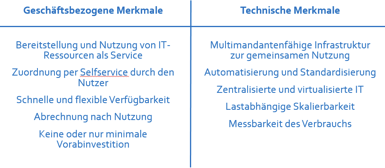
\includegraphics[width=0.7\linewidth]{screenshot003}
	\caption{}
	\label{fig:screenshot003}
\end{figure}

\subsection*{Frage 3}
Nennen und erläutern Sie die 3 Betriebsarten von Cloud Computing!
\subsection*{Antwort}
\begin{itemize}
	\item Public Cloud
	\item Private Cloud
	\item Hybrid Cloud ( Mischung aus P und P)
\end{itemize}
\subsection*{Frage 4}
Nennen Sie die 3 Arten von Cloud-Angeboten (3-Ebenen-Modell)!
\subsection*{Antwort}
\begin{itemize}
	\item IaaS
	\item PaaS
	\item SaaS
\end{itemize}
\subsection*{Frage 5}
Was sind die wesentlichen Vorteile von PaaS im Vergleich zur klassischen Entwicklung von Anwendungen?
\subsection*{Antwort}
\begin{itemize}
	\item Beschleunigung von Geschäftsprozessen
	\item Schnelleres und flexibleres Testen und Entwickeln
	\item Ideales Werkzeug für agile Entwicklung / DevOps
\end{itemize}
\subsection*{Frage 6}
Welche Möglichkeiten zur Skalierung gibt es bei IBM Bluemix?
\subsection*{Antwort}
\begin{itemize}
	\item Manuelle Skalierung 
	\item Automatische Skalierung der Instanzen anhand von festgelegten Regeln
\end{itemize}
